% !TeX root = ../presentation.tex

\section{Vision}

% TODO: Vis., Beispiele

\begin{frame}{Strategische Ressource {\footnotesize\cite{mollerIndustrialDataEcosystems2024}}}
    \begin{columns}
        \begin{column}{0.7\textwidth}
            \begin{itemize}
                \item Daten: vom \enquote{Nebenprodukt} zur strategischen Ressource
                \item Datenaustausch essenziell für Geschäftsprozesse
                \item Koordination von Lieferketten, Erfüllung rechtlicher Rahmenbedingungen
                
                \item<2-> viele Bedenken beim Data Sharing
                \begin{itemize}
                    \item<2-> Missbrauch von Daten
                    \item<3-> Angst vor unberechtigter Weitergabe
                \end{itemize}

                \note{
                    \begin{itemize}
                        \item Angst vor unberechtigte Weitergabe: Geschäftsgeheimnisse
                    \end{itemize}
                }
                
                \item<4-> meist nur bilateraler, eingeschränkter Datenaustausch
                
                \item[$\Rightarrow$]<5-> vertrauensvolles, multilaterales Data Sharing
            \end{itemize}
        \end{column}

        \begin{column}{0.3\textwidth}
            \begin{figure}
                \centering
                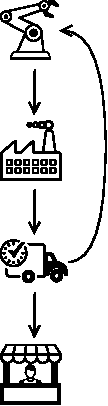
\includegraphics[height=6cm]{./assets/supply_chain.drawio.pdf}
                \caption{Lieferkette}
            \end{figure}
        \end{column}
    \end{columns}
\end{frame}


\begin{frame}{Aufwendige Datenintegration}
    \begin{columns}
        \begin{column}{0.7\textwidth}
            \begin{itemize}
                \item Datenintegration $\to$ Optimierung von Geschäftsprozessen
                \item Integration mehrerer Projekte oft mittels\\
                    \emph{Extract, Transform, Load}
                \item wiederholte Schritte, zeitintensiv, teuer, inkonsistent
                \item hohe Einstiegsbarriere für neue Akteure
        
                \item[$\Rightarrow$]<2-> schnelles, effizientes, günstiges Verfahren
                \item[$\Rightarrow$]<2-> Datenkonsistenz
                \item[$\Rightarrow$]<2-> Begünstigung innovativer Lösungen
            \end{itemize}
        \end{column}

        \begin{column}{0.3\textwidth}
            \addtocounter{figure}{-1}
            \begin{figure}
                \centering
                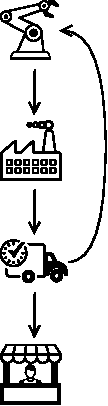
\includegraphics[height=6cm]{./assets/supply_chain.drawio.pdf}
                \caption{Lieferkette}
            \end{figure}
        \end{column}
    \end{columns}
\end{frame}


\begin{frame}{Datensilos und Datensouveränität}
    \begin{columns}
        \begin{column}{0.65\textwidth}
            \begin{itemize}
                \item Daten als wertvolles Wirtschaftsgut $\to$ Datensilos
                \item mangelnde Privatsphäre und Kontrolle
                \begin{itemize}
                    \item[$\to$] zurückhaltendes Data Sharing
                \end{itemize}
                \item mangelnde Kooperation
                \begin{itemize}
                    \item[$\to$] mehrfache Speicherung derselben Daten
                    \item[$\to$] veraltete, inkonsistente Daten
                \end{itemize}
        
                \item[$\Rightarrow$]<2-> Verfügbarkeit von aktuellen, konsistenten Daten
                \item[$\Rightarrow$]<2-> Datenschutz \emph{und} Datensouveränität
            \end{itemize}
        \end{column}

        \begin{column}{0.35\textwidth}
            \vspace{2em}
            \begin{figure}
                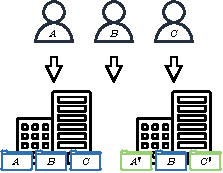
\includegraphics[width=\textwidth]{./assets/central.drawio.pdf}
                \caption{Zentralisierte Datenspeicherung}
            \end{figure}
        \end{column}
    \end{columns}

    \note{
        \begin{itemize}
            \item mehrfache Speicherung derselben Daten\\
                $\to$ dasselbe in grün, aber es ist nicht dasselbe, sondern etwas veraltetes
            \\~\\
            \item Bild: Bsp: nach Umzug bei jedem Arzt neue Adresse angeben
        \end{itemize}
    }
\end{frame}
